\chapter{DUST solver}

The DUST solver is the main executable of DUST, and its aim is to run 
the actual simulation and obtain the required full solution to the problem. 

As the other executable it is run by simply invoking the executable \texttt{dust} with the correct input file as command argument.
\begin{command}[caption={Solver command looking for input file 
    \texttt{input\_file\_name.in}}]
    dust input_file_name.in
\end{command}

If no command argument is provided the solver looks for a default input file, \texttt{dust.in}. 
\begin{command}[caption={Solver command looking for 
default input file \texttt{dust.in}}]
    dust
\end{command}

The solver requires, among other inputs, the geometry file result of the preprocessor. 
If such file is not found the solver attempts to run the preprocessor by executing 
the preprocessor with default input file (command \ref{command:dus_pre_default}). 

\section{Input file}
\label{sec:Solver_InputFile}

The input file which should be provided to the solver is used to set all t
he parameters required for the execution of the simulation, 
from execution options, time parameters to the wake and model 
settings. 

An example of input file for the solver is presented in file \ref{file:dust.in}

\begin{inputfile}[frame=single, caption={dust.in}, label={file:dust.in}]

! --- execution parameters ---
basename = sim_01
basename_debug = sim_01_debug
debug_level = 3

! --- time parameters ---
tstart = 0.0
tend = 10.0
timesteps = 20
!dt = 0.5
dt_out = 2.0
dt_debug_out = 1.0
output_start = F
output_detailed_geo = T 

! --- restart parameters ---
restart_from_file = F
restart_file = prev_solution_0021.h5
reset_time = F

! --- input files ---
reference_file = References.in
geometry_file = geo_file.h5

! --- stream parameters ---
u_inf = (/1.0, 0.0, 0.0/)
u_ref = 1.0
P_inf = 1.0
rho_inf = 1.0
a_inf = 340.0
mu_inf = 0.00001

! --- wake parameters ---
n_wake_panels = 4
n_wake_particles = 10000
particles_box_min = (/-10.0, -10.0, -10.0/)
particles_box_max = (/10.0, 10.0, 10.0/)
implicit_panel_scale = 0.3
implicit_panel_min_vel = 1.0e-8
rigid_wake = F
rigid_wake_vel = (/1.0, 0.0, 0.0/)
join_te = F
join_te_factor = 1.0

! --- model parameters ---
far_field_ratio_doublet = 10.0
far_field_ratio_source = 10.0
doublet_threshold = 1.0e-6
rankine_rad = 0.1
vortex_rad = 0.1
k_vortex_rad = 1.0
cutoff_rad = 0.001

! --- additional models to use ---
vortstretch = T
vortstretch_from_elems = F
diffusion = T
turbulent_viscosity = F
penetration_avoidance = F
penetration_avoidance_check_radius = 5.0
penetration_avoidance_element_radius = 1.5
divergence_filtering = T
filter_time_scale = 40.0
fmm = T
fmm_panels = F
viscosity_effects = F
particles_redistribution = F
particles_redistribution_ratio = 3.0
octree_level_solid = 4
turbulent_viscosity = F
HCAS = F
HCAS_time = 4.0
HCAS_velocity = (/2.0, 0.0, 0.0/)

! --- Fast multipole parameters ---
box_length = 10.0
n_box = (/2, 2, 2/)
octree_origin = (/-10.0, -10.0, -10.0/)
n_octree_levels = 6
min_octree_part =  10
multipole_degree = 2
dyn_layers = F
nmax_octree_levels = 7
leaves_time_ratio = 3.0

! --- Lifting Lines parameters ---
ll_solver = GammaMethod
ll_reynolds_corrections = F
ll_reynolds_corrections_nfact = 0.2
ll_max_iter = 100
ll_tol = 1.0e-6
ll_damp = 5.0
ll_stall_regularisation = T
ll_stall_regularisation_nelems = 1
ll_stall_regularizations_niters = 1
ll_stall_regularization_alpha_stall = 15
ll_artificial_viscosity = 0.0
ll_artificial_viscosity_adaptive = F
ll_artificial_viscosity_adaptive_alpha = 15
ll_artificial_viscosity_adaptive_dalpha = 3
ll_loads_avl = F

! --- Vortex Lattice Correction ---
vl_tol = 1.0e-4
vl_relax = 0.3
vl_maxiter = 100
vl_start_step = 0
vl_dynstall = F
aitken_relaxation = T 

\end{inputfile}

The details of each parameter are:
\begin{itemize}
\item \param{basename}: \textit{required:} yes. \textit{multiple:} no. \textit{type:} string.

The base name of the simulation and will be the prefix of the output files. 
Can be a complete path leading to the location in which to store the results. 

\item \param{basename\_debug}: \textit{required:} no. \textit{multiple:} no. 
\textit{default:} \param{basename} \textit{type:} string.

The base name of the debug output. It is especially useful to direct the 
debug output to a different location than the standard output. 
The amount of (if any) debug output is controlled by \param{debug\_level}.

\item \param{debug\_level}: \textit{required:} no. \textit{multiple:} no. 
\textit{default:} 1\textit{type:} integer.

A parameter controlling the verbosity (both in terms of standard output and files output) 
of the simulation. A smaller value leads to fewer output, with 0 being a silent simulation, 
while values higher of 10 lead to debug files to be produced. 
A value of 3 is a balanced value to obtain a reasonable amount of informations 
on the simulation. 

WARNING: the present feature tends to evolve rapidly during the development. 
Values higher than 10 may lead to unexpected behaviours. 


\item \param{tstart}: \textit{required:} yes. \textit{multiple:} no. \textit{type:} real.

The start time of the simulation.

\item \param{tend}: \textit{required:} yes. \textit{multiple:} no. \textit{type:} real.

The end time of the simulation.

\item \param{timesteps}: \textit{required:} yes if \param{dt} not set, forbidden if set. 
\textit{multiple:} no. \textit{type:} integer.

The number of timesteps for the simulation. Note that during the simulation a number 
of timesteps equal to \param{timesteps}+1 will be displayed, because the starting step 
is counted too. 

\item \param{dt}: \textit{required:} yes if \param{timesteps} not set, forbidden if set. 
\textit{multiple:} no. \textit{type:} real.

The time step length.

\item \param{dt\_out}: \textit{required:} yes. \textit{multiple:} no. \textit{type:} real.

Time interval of solution output.

\item \param{dt\_debug\_out}: \textit{required:} no. \textit{multiple:} no. \textit{default:} 
\param{dt\_out}. \textit{type:} real.

Time interval of debug output, if \param{debug\_level} is set high enough to write debug 
files.


\item \param{output\_start}: \textit{required:} no. \textit{multiple:} no. 
\textit{default} False. \textit{type:} logical.

Output the first iteration. Since it is an implicit solver, the first calculation happens 
at $t_0$ before any time interval has passed, if set to True output the first result.

\item \param{output\_detailed\_geo}: \textit{required:} no. \textit{multiple:} no. 
\textit{default} False. \textit{type:} logical.

Output additional geometry information in the result files. Makes the result files 
easier to interpret by third party software, however makes the result files slightly 
bigger and output slightly slower.

\item \param{restart\_from\_file}: \textit{required:} no. \textit{multiple:} no. 
\textit{default:} False. \textit{type:} logical.

Restart the simulation from a previous result.


\item \param{restart\_file}: \textit{required:} yes if \param{restart\_from\_file} 
is true. \textit{multiple:} no. \textit{type:} string.

name of the solution file from which to restart the simulation.

Note: when reloading a certain result, the solver will attempt to load also the 
relative geometry file in the same location, as discussed in \ref{sec:Solver_Output_Files}. 
If such geometry file is not provided the solver, as in the case of standard starting, 
will attempt to generate such file with the default preprocessor input. Beware that in 
this case, if the geometry of the results from which the solver is starting was generated 
from another geometry input this could lead to unexpected behaviour.


\item \param{reset\_time}: \textit{required:} no. \textit{multiple:} no. \textit{default:} 
False. \textit{type:} logical.

If set to true, when restarting from a previous result, the time will be set as the 
\param{tstart} from the input file. If set to false, the time will be set as the one 
from the result file loaded. This is delicate since the movement of the reference 
frames is based on the current time in the simulation, and if reset the time could 
lead to a position of the geometry different from the one in the loaded result file.


\item \param{reference_file}: \textit{required:} yes. \textit{multiple:} no. 
\textit{type:} string.

name of the file containing the definition of the reference frames employed 
in the simulation.


\item \param{geometry_file}: \textit{required:} yes. \textit{multiple:} no. 
\textit{type:} string.

name of the file containing the geometry definition, generated by the preprocessor


\item \param{u\_inf}: \textit{required:} no. \textit{multiple:} no. 
\textit{default:} (/1.0, 0.0, 0.0/) \textit{type:} real array of length 3.

Free stream velocity vector.

\item \param{u\_ref}: \textit{required:} no. \textit{multiple:} no. 
\textit{default:} $|\text{\param{u\_inf}}|$ \textit{type:} real.

Reference velocity. Usually is safe not to set anything and use the norm 
of the free stream velocity, however in hover flight conditions it is useful 
to set a non zero reference velocity (e.g. the blade tip velocity)


\item \param{gust}: \textit{required:} no. \textit{multiple:} no. 
\textit{default:} F \textit{type:} logical.

\begin{itemize}
    
    \item \param{gust_type}: \textit{required:} no. \textit{multiple:} no. \textit{default:} AMC \textit{type:} string.
    
    Select the gust type: \opt{ACM} or \opt{linear}.
    \begin{equation}
        \vec{s} = -\sum \big[\vec{x} - \big(\vec{O} + U_{des}\vec{v}(t-\tau)\big)\vec]\vec{v}
    \end{equation}
        
    \begin{equation}
        \vec{U} = \vec{U}  + \dfrac{U_{des}}{2}\bigg(1-\cos{\frac{\pi s}{H}}\bigg)    
    \end{equation}
    
    \item \param{gust_origin}: \textit{required:} yes. \textit{multiple:} no. 
    \textit{type:} real array of length 3.
    
    $\vec{0}$: Position of the point  whose airstream velocity is being computed. 
    
    \item \param{gust_front_direction}: \textit{required:} yes. \textit{multiple:} no. 
    \textit{type:} real array of length 3.
    
    $\vec{v}$: Unit vector that defines the direction of propagation of the front. 
    
    \item \param{gust_front_speed}: \textit{required:} yes. \textit{multiple:} no. 
    \textit{type:} real.
    
    Velocity of propagation of the front in direction 
    \param{gust_front_direction}
    
    \item \param{gust_u_des}: \textit{required:} yes. \textit{multiple:} no. 
    \textit{type:} real.
    
    $U_{des}$: gust amplitude. 
    
    \item \param{gust_perturbation_direction}: \textit{required:} no. 
    \textit{multiple:} no. \textit{default:} (/0.0, 0.0, 1.0/) 
    \textit{type:} real array of length 3.
    
    Unit vector that defines the direction of the velocity perturbation
    
    \item \param{gust_gradient}: \textit{required:} no. \textit{multiple:} yes. 
    \textit{type:} real.
    
    H: gust wave length. 
    
    \item \param{gust_start_time}: \textit{required:} no. \textit{multiple:} no. 
    \textit{default:} 0.0 \textit{type:} real.
    
    $\tau$: Time at which the gust starts. 
\end{itemize}

\item \param{P\_inf}: \textit{required:} no. \textit{multiple:} no. 
\textit{default:} 101325.0 \textit{type:} real.

Free stream pressure.

\item \param{a\_inf}: \textit{required:} no. \textit{multiple:} no. 
\textit{default:} 340.0 \textit{type:} real.

Free stream sound speed. For lifting lines and compressibility corrections.


\item \param{mu\_inf}: \textit{required:} no. \textit{multiple:} no. 
\textit{default:} 0.000018 \textit{type:} real.

Free stream dynamical viscosity. For lifting lines and viscosity corrections.

\item \param{rho\_inf}: \textit{required:} no. \textit{multiple:} no. 
\textit{default:} 1.225 \textit{type:} real.

Free stream density.

\item \param{n\_wake\_panels}: \textit{required:} no. \textit{multiple:} no. 
\textit{default:} 1 \textit{type:} integer.

Number of panel wake rows before converting the wake to vortex particles.


\item \param{n\_wake\_particles}: \textit{required:} no. \textit{multiple:} no. 
\textit{default:} 10000 \textit{type:} integer.

Number of maximum vortex particles in the wake. If the limit is reached the simulation is stopped, but can be restarted from last save with a higher value of the parameter. 


\item \param{particles\_box\_min}: \textit{required:} no. \textit{multiple:} no. 
\textit{default:} (/-10.0, -10.0, -10.0/) \textit{type:} real array of length 3.

Minimum coordinates (in the base reference frame) of the box containing the vortex 
particles. If the particles get outside the box are cancelled.

\item \param{particles\_box\_max}: \textit{required:} no. \textit{multiple:} no. 
\textit{default:} (/10.0, 10.0, 10.0/) \textit{type:} real array of length 3.

Maximum coordinates (in the base reference frame) of the box containing the vortex 
particles. If the particles get outside the box are cancelled.

\item \param{implicit_panel_scale}: \textit{required:} no. \textit{multiple:} no. 
\textit{default:} 0.3 \textit{type:} real.

Scaling of the first panel of the wake, the implicit one which enforces the Kutta 
condition. The first panel geometry is not dictated by the advection of its 
vertices as for the other ones, but the first row of points come from the geometry, 
while the second row is calculated by local velocity and timestep, 
scaled by the \param{implicit_panel_scale} parameter.


\item \param{implicit_panel_min_vel}: \textit{required:} no. \textit{multiple:} no. 
\textit{default:} 1.0e-8 \textit{type:} real.

When the free stream velocity and body motions do not create a sufficiently high 
local velocity at the trailing edge, the first panel might turn out of zero length. 
To avoid this, when the trailing edge local velocity is below 
\param{implicit_panel_min_vel} a fixed length of the panel is imposed.

\item \param{rigid\_wake}: \textit{required:} no. \textit{multiple:} no. 
\textit{default:} False \textit{type:} logical.

Impose a wake which is evolved rigidly according to a prescribed global 
velocity rather than the local velocity field. Works for both panels and 
particles.

\item \param{rigid\_wake\_vel}: \textit{required:} yes if \param{rigid\_wake} is True. 
\textit{multiple:} no. \textit{type:} real array of length 3.

Velocity to impose to the rigid wake.

\item \param{join\_te}: \textit{required:} no. \textit{multiple:} no. 
\textit{default:} False. \textit{type:} logical.

Employ trailing edge joining for close trailing edges.

\item \param{join\_te\_factor}: \textit{required:} no. \textit{multiple:} no. 
\textit{default:} 1.0. \textit{type:} real.

If employing joining of trailing edges, the trailing edges which are closer than 
\param{join\_te\_factor} times the length of the adjacent trailing edge elements 
will be joined. 

\item \param{far_field_ratio_doublet}: \textit{required:} no. \textit{multiple:} no. 
\textit{default:} 10.0 \textit{type:} real.

Ratio with respect to element length to set the thresholds for far field approximation. 
When evaluating the influence of the doublets of an element, 
if the evaluation point is distant more than \param{far_field_ratio_doublet} 
times the characteristic length of the element, simplified cheaper far field 
approximated formulae are employed instead of the standard ones. 
The characteristic length of the element is taken as the maximum 
length of all the element edges.

\item \param{far_field_ratio_source}: \textit{required:} no. 
\textit{multiple:} no. \textit{default:} 10.0 \textit{type:} real.

As for \param{far_field_ratio_doublet} determines the threshold 
after which far field approximations are employed, just for sources. 
Applies only to three dimensional surface panels. 

\item \param{doublet_threshold}: \textit{required:} no. \textit{multiple:} no. 
\textit{default:} 1.0e-6 \textit{type:} real.

Parameter which sets the distance threshold under which the evaluation point, 
with respect to a panel, is considered inside the plane of the panel.

\item \param{rankine_rad}: \textit{required:} no. \textit{multiple:} no. 
\textit{default:} 0.1 \textit{type:} real.

Parameter which sets the radius under which the Rankine approximation of 
vortexes cores is employed. Used for aerodynamic elements and panels 
(i.e. everything except vortex particles)

\item \param{vortex_rad}: \textit{required:} no. \textit{multiple:} no. 
\textit{default:} 0.1 \textit{type:} real.

Parameter which uniformly sets the radius of the vortex particles, only used if \param{k_vortex_rad} is disabled.

\item \param{k_vortex_rad}: \textit{required:} no. \textit{multiple:} no. \textit{default:} 1.0 \textit{type:} real.

Coefficient for the automatic computation of the radius of each vortex particle; set a negative number to disable the feature and revert to uniform vortex radius. 

\item \param{cutoff_rad}: \textit{required:} no. \textit{multiple:} no. 
\textit{default:} 0.001 \textit{type:} real. 

Parameter which sets the radius under which the vortexes interaction is completely set to zero.

\item \param{vortstretch}: \textit{required:} no. \textit{multiple:} no. 
\textit{default:} T \textit{type:} logical.

Calculate the evolution of vorticity of the particles considering the 
vortex stretching

\item \param{vortstretch_from_elems}: \textit{required:} no. 
\textit{multiple:} no. \textit{default:} F \textit{type:} logical.

Compute also the contribution to the vortex stretching of the particles 
due to the model elements. 

\item \param{diffusion}: \textit{required:} no. \textit{multiple:} no. 
\textit{default:} T \textit{type:} logical.

Calculate the evolution of vorticity of the particles considering the vorticity diffusion

\item \param{turbulent_viscosity}: \textit{required:} no. \textit{multiple:} no. 
\textit{default:} F \textit{type:} logical.

Introduce additional turbulent viscosity (Smagorinsky style) to the vorticity 
diffusion term. Working only when \param{fmm} is turned on. Still experimental feature. 

\item \param{penetration_avoidance}: \textit{required:} no. \textit{multiple:} no. 
\textit{default:} F \textit{type:} logical.

Apply the penetration avoidance algorithm to avoid the penetration of particles 
inside the solid bodies.

\item \param{penetration_avoidance_check_radius}: \textit{required:} no. 
\textit{multiple:} no. \textit{default:} 5.0 \textit{type:} real.

radius multiplication factor of the check radius. All the particles within a 
distance $d\leq P_r U_{ref} \Delta t$ from each element are checked for 
potential penetration, where $P_r$ is the multiplication factor. 
A bigger factor minimizes the risk of penetration of extremely fast particles, 
but affects the performance. 

\item \param{penetration_avoidance_element_radius}: \textit{required:} no. 
\textit{multiple:} no. \textit{default:} 1.5 \textit{type:} real.

Surface correction element radius multiplication factor.
The velocity of the particles is corrected to avoid penetration through a 
particular element if the particle hits the surface within a distance 
(tangent to the surface) $d_t \leq P_e \max{l_i} \frac{\sqrt{2}}{2}$ 
from the element centre, where $l_i$ are the lenght of the element sides 
and $P_e$ is the factor. 
A bigger factor leads to a potentially higher level of correction 
(concurrent correction from different neighbouring elements) 
while a smaller factor may let some particles slip through the surface. 

\item \param{divergence_filtering}: \textit{required:} no. \textit{multiple:} no. 
\textit{default:} T \textit{type:} logical.

Employ the divergence filtering to keep the vorticity field divergence-free. 

\item \param{filter_time_scale}: \textit{required:} no. \textit{multiple:} no. 
\textit{default:} 40.0 \textit{type:} real.

Timescale of the time filter to filter the divergence. 
The input is not the actual timescale but the number of simulation timesteps 
of which the timescale is consisting. 

\item \param{fmm}: \textit{required:} no. \textit{multiple:} no. \textit{default:} T 
\textit{type:} logical.

Use the fast multipole method for particles evolution.

\item \param{fmm_panels}: \textit{required:} no. \textit{multiple:} no. 
\textit{default:} F \textit{type:} logical.

Use the fast multipole method also to compute interactions 
of the particles on the solid bodies panels.

\item \param{viscosity_effects}: \textit{required:} no. \textit{multiple:} no. 
\textit{default:} F \textit{type:} logical.

Take into account viscosity effects on the geometry surface: 
enables the release of vortex particles from different points 
on the geometry surface. Experimental feature, still in development.

\item \param{particles_redistribution}: \textit{required:} no. 
\textit{multiple:} no. \textit{default:} F \textit{type:} logical.

Redistribute the particles having a small intensity to the neighbouring ones. 
Active only if \param{fmm} is active, otherwise ignored. Redistributed particles 
are then ereased to reduce the total number of particles.

\item \param{particles_redistribution_ratio}: \textit{required:} no. 
\textit{multiple:} no. \textit{default:} 3.0 \textit{type:} real.

When employing \param{particles_redistribution}, each particle of intensity 
$|\vec{\alpha}_i|$ will be redistributed to the other particles contained 
in the octree leaf cell if $|\vec{\alpha}_i| r < \alpha_{ave}$ where $r$ is 
\param{particles_redistribution_ratio} and $\alpha_{ave}$ is the average 
intensity of the particles inside the cell.

\item \param{octree_level_solid}: \textit{required:} yes, if 
\param{particles_redistribution} is true. \textit{multiple:} no. 
\textit{type:} integer.

When employing \param{particles_redistribution}, the particles too near 
to a solid boundary are not redistributed to reduce the error induced by 
the redistribution on the solution on solid surfaces. The octree cells at 
level \param{octree_level_solid} containing a panel (SP, VL or LL) are marked 
as containing a solid boudary, as well as all their neighbour at that level. 
All the children of cells containing a solid boundary are marked as containing 
a solid boundary. In the cells containing a solid boundary the redistribution 
is not performed.

For this reason, a small \param{octree_level_solid} approaching 1 will lead 
to a wide zone around solid bodies in which redistribution does not occur, 
while a \param{octree_level_solid} approaching \param{n_octree_levels} leads 
to redistribution to be performed in areas up to close to the solid bodies.

\item \param{turbulent_viscosity}: \textit{required:} no. \textit{multiple:} no. 
\textit{default:} F \textit{type:} logical.

Employ an additional turbulent viscosity, using a Smagorinsky-like model to 
take into account the dissipation of energy in turbulent conditions towards 
small, not resolved turbulent scales. It works only in an octree environment, 
so when \param{fmm} is active.

\item \param{HCAS}: \textit{required:} no. \textit{multiple:} no. 
\textit{default:} F \textit{type:} logical.

Hover Convergence Augmentation System. An additional velocity is applied 
to the particles in the wake to let the particles generated in the transient 
condition at the start to be pushed faster outside the domain, and reach 
stationary conditions faster. The velocity defined by \param{HCAS\_velocity} 
is applied full only at the beginning of the simulation, and is then decreased 
linearly in \param{HCAS\_time}. After \param{HCAS\_time} after the simulation 
start the additional velocity is not applied anymore and the simulation carries 
on without tampering. 

\item \param{HCAS\_time}: \textit{required:} yes if \param{HCAS} is true. 
\textit{multiple:} no. \textit{type:} real.

Duration of HCAS application

\item \param{HCAS\_velocity}: \textit{required:} yes if \param{HCAS} is true. 
\textit{multiple:} no. \textit{type:} real array of length 3.

Velocity to apply to the particles during the HCAS use. 

\item \param{box_length}: \textit{required:} yes if \param{fmm} is true. 
\textit{multiple:} no. \textit{type:} real.

Length of the level 1 cubic boxes composing the octree. See figure 
\ref{fig:boxes1} for a graphic explanation.

\item \param{n_box}: \textit{required:} yes if \param{fmm} is true. 
\textit{multiple:} no. \textit{type:} integer array of length 3.

Number of base level 1 cubic boxes in each spatial direction. See figure 
\ref{fig:boxes1} for a graphic explanation.

\item \param{octree_origin}: \textit{required:} yes if \param{fmm} is true. 
\textit{multiple:} no. \textit{type:} real array of length 3. 

origin of the octree. Starting from the origin, the octree mesh extends in 
each direction of \param{n_box} times \param{box_length}. 
See figure \ref{fig:boxes1} for a graphic explanation.

\item \param{n_octree_levels}: \textit{required:} yes if \param{fmm} is true. 
\textit{multiple:} no. \textit{type:} integer.

Number of levels in  which the base boxes are divided. At each level 
the upper level boxes are divided into eight half sized boxes. 

\item \param{min_octree_part}: \textit{required:} yes if \param{fmm} is true. 
\textit{multiple:} no. \textit{type:} integer.

Minimum number of particles contained in an octree box in order to consider 
it a leaf (lowest level box). If not enough particles are contained in a 
box, the box is not considered and the particles are gathered at the higher 
level parent box.

\item \param{multipole_degree}: \textit{required:} yes if \param{fmm} is true. 
\textit{multiple:} no. \textit{type:} integer.

Degree of the expansions in the multipole method. 

\item \param{dynamic_layers}: \textit{required:} no. \textit{multiple:} no. 
\textit{default:} False. \textit{type:} logical.

Use dynamic octree layers, i.e. a further division layer in the octree 
is added every time the time spent in the particle to particle calculations 
is greater than the one spent in the fast multipole part.

\item \param{nmax_octree_levels}: \textit{required:} yes if \param{dynamic_layers} is True. 
\textit{multiple:} no. \textit{type:} integer.

Maximum number of divisions allowed during dynamic layers. The number of starting 
layers is still \param{n_octree_levels}, which however might increase during the 
simulation, but are always kept under a maximum number. 

WARNING: it is advised not to let the number of octree layers to be greater than 7. 
The number of cells in the octree increases really rapidly at each subdivision, 
and after 7 layers it is easy to fill the complete memory just with the pointers 
necessary to keep the track of the connectivity. 

\item \param{leaves_time_ratio}: \textit{required:} yes if \param{dynamic_layers} is True. 
\textit{multiple:} no. \textit{type:} real.

Ratio between the time spent in the particle to particle computations in the 
leaves of the octree with respect to the rest of the fast multipole computations 
that triggers the increase of the octree levels.

\item \param{ll_solver}: \textit{required:} no. \textit{multiple:} no. 
\textit{default:} \opt{GammaMethod}. \textit{type:} string.

Choose the type of lifting line solver to be employed. 
\opt{gammma_method} performs a fixed point iteration method with the lifting 
line circulation as the unknown variable. It is the default method. 

\opt{alpha_method} performs a similar fixed point method but with the angle 
of attack of the lifting line section as variable. 
It allows for the use of regularization in case of problematic 
partially stalled configurations. 

\item \param{ll_reynolds_corrections}: \textit{required:} no. 
\textit{multiple:} no. \textit{default:} False. \textit{type:} logical.

Employ a Reynolds number correction to obtain an extrapolation of 
the lifting lines tables at the simulation conditions Reynolds number 
if different than the one(s) provided in the lookup tables

\item \param{ll_reynolds_corrections_nfact}: \textit{required:} no. 
\textit{multiple:} no. \textit{default:} 0.2 \textit{type:} real.

The Reynolds correction extrapolation is based on a power law: 
$Cf = Cf_T \left(\frac{Re}{Re_T}\right)^N$, the parameter provides the 
value of the power law. Usually it can vary from 0.125 to 0.2.

\item \param{ll_max_iter}: \textit{required:} no. \textit{multiple:} no. 
\textit{default:} 100 \textit{type:} integer.

Number of iterations of the fixed point non-linear solver used to obtain 
the lifting lines solution.

\item \param{ll_tol}: \textit{required:} no. \textit{multiple:} no. 
\textit{default:} 1.0e-6 \textit{type:} real.

Relative tolerance at which the fixed point lifting lines solver stops

\item \param{ll_damp}: \textit{required:} no. \textit{multiple:} no. 
\textit{default:} 25.0 \textit{type:} real.

Value of the damping (relaxation) coefficient employed during fixed point 
iterations, to suppress possible oscillations.

\item \param{ll_stall_regularisation}: \textit{required:} no. 
\textit{multiple:} no. \textit{default:} True. \textit{type:} logical.

During the first timesteps of simulations employing lifting lines, 
usually in challenging configurations such as hovering rotors, 
it is possible that a non perfect convergence of the non-linear 
solver leads to some few elements of the lifting line (typically one) 
to converge on a stalled configuration among a series of completely 
non stalled elements. This is unphysical, and usually it is solved 
during the evolution of the simulation. It is however possible to 
identify this behaviour and use the previous solution for these 
sections to improve convergence. 

\item \param{ll_stall_regularisation_nelems}: \textit{required:} no. 
\textit{multiple:} no. \textit{default:} 1. \textit{type:} integer.

Number of lifting line elements to correct in case of isolated 
stall among non stalled elements. At the moment cannot be higher than 1.

\item \param{ll_stall_regularisation_niters}: \textit{required:} no. 
\textit{multiple:} no. \textit{default:} 1. \textit{type:} integer.

Number of LL iterations between two regularisation processes.

\item \param{ll_stall_regularisation_alpha_stall} \textit{required:} no. 
\textit{multiple:} no. \textit{default:} 15.0. \textit{type:} real.

Stall angle [deg] used as a threshold for regularisation process. 

\item \param{ll_loads_avl}: \textit{required:} no. \textit{multiple:} no. 
\textit{default:} F. \textit{type:} logical.

Use AVL expression for the inviscid load contributions of LL elements, 
in the same way of load computation used for VL elements. 

\item \param{ll_artificial_viscosity}: \textit{required:} no. 
\textit{multiple:} no. \textit{default:} 0.0. \textit{type:} real.

Artificial viscosity used to spatially regularize the solution with 
a gaussian kernel, to be used in case of \param{ll_solver} = \opt{alpha_method} 
to regularize post-stall situations. The default value of 0 leads to no 
regularization, while values greater than 0 lead to wider gaussian regularization. 
The value is uniform in the domain if \param{ll_artificial_viscosity_adaptive} is 
false, while if true represents the maximum introduced value.

\item \param{ll_artificial_viscosity_adaptive}: \textit{required:} no. 
\textit{multiple:} no. \textit{default:} False. \textit{type:} logical.

Use an adaptive strategy to introduce artificial viscosity for regularization, 
in order to regularize post stall configuration while not influencing non 
stalled configurations. 

\item \param{ll_artificial_viscosity_adaptive\_alpha}: \textit{required:} yes if 
\param{ll_artificial_viscosity_adaptive} is true. \textit{multiple:} no. \textit{type:} real.

Angle of attack after which the full artificial viscosity is introduced, 
thus after which the maximum regularization is operated. Should be set 
around or over the stall angle

\item \param{ll_artificial_viscosity_adaptive\_dAlpha}: \textit{required:} 
yes if \param{ll_artificial_viscosity_adaptive} is true. \textit{multiple:} no. 
\textit{type:} real.

Angle of attack range before \param{ll_artificial_viscosity_adaptive\_alpha} 
where the artificial viscosity is gradually introduced from zero to the maximum 
value set in \param{ll_artificial_viscosity}.

\item \param{vl_tol}: \textit{required:} no. \textit{multiple:} no. 
\textit{default:} 1.0e-4 \textit{type:} real. 
Tolerance for the absolute error on lift coefficient in fixed point 
iteration for corrected vortex lattice.

\item \param{vl_relax}: \textit{required:} no. \textit{multiple:} no. 
\textit{default:} 0.3 \textit{type:} real. 
Constant relaxation factor for rhs update

\item \param{aitken_relaxation}: \textit{required:} no. \textit{multiple:} no. 
\textit{default:} T \textit{type:} logical. 
Activate the Aitken acceleration and stabilization method involved during the 
vortex lattice fixed point iteration. 
The initial relaxation is the one specified in \opt{vl_relax}. 

\item \param{vl_maxiter}: \textit{required:} no. \textit{multiple:} no. 
\textit{default:} 100 \textit{type:} integer. 
Max number of iteration for correction of vortex lattice

\item \param{vl_start_step}: \textit{required:} no. \textit{multiple:} no. 
\textit{default:} 1 \textit{type:} integer. 
Time step to start correcting the vortex lattice element

\item \param{vl_dynstall}: \textit{required:} no. \textit{multiple:} no. 
\textit{default:} F \textit{type:} logical. 
Activate Boeing\footnote{\url{https://apps.dtic.mil/sti/pdfs/AD0767240.pdf}} 
dynamic stall on the corrected \param{v} element.  (Still experimental)

\item \param{vl_average}: \textit{required:} no. \textit{multiple:} no. 
\textit{default:} F \textit{type:} logical. 
Average the solution between the iteration: this may further stabilize the solution in stalled conditions

\item \param{vl_average_iter}: \textit{required:} no. \textit{multiple:} no. 
\textit{default:} 10 \textit{type:} integer. 
Number of iteration on which the average is computed. 

\end{itemize}

\begin{figure}
\centering
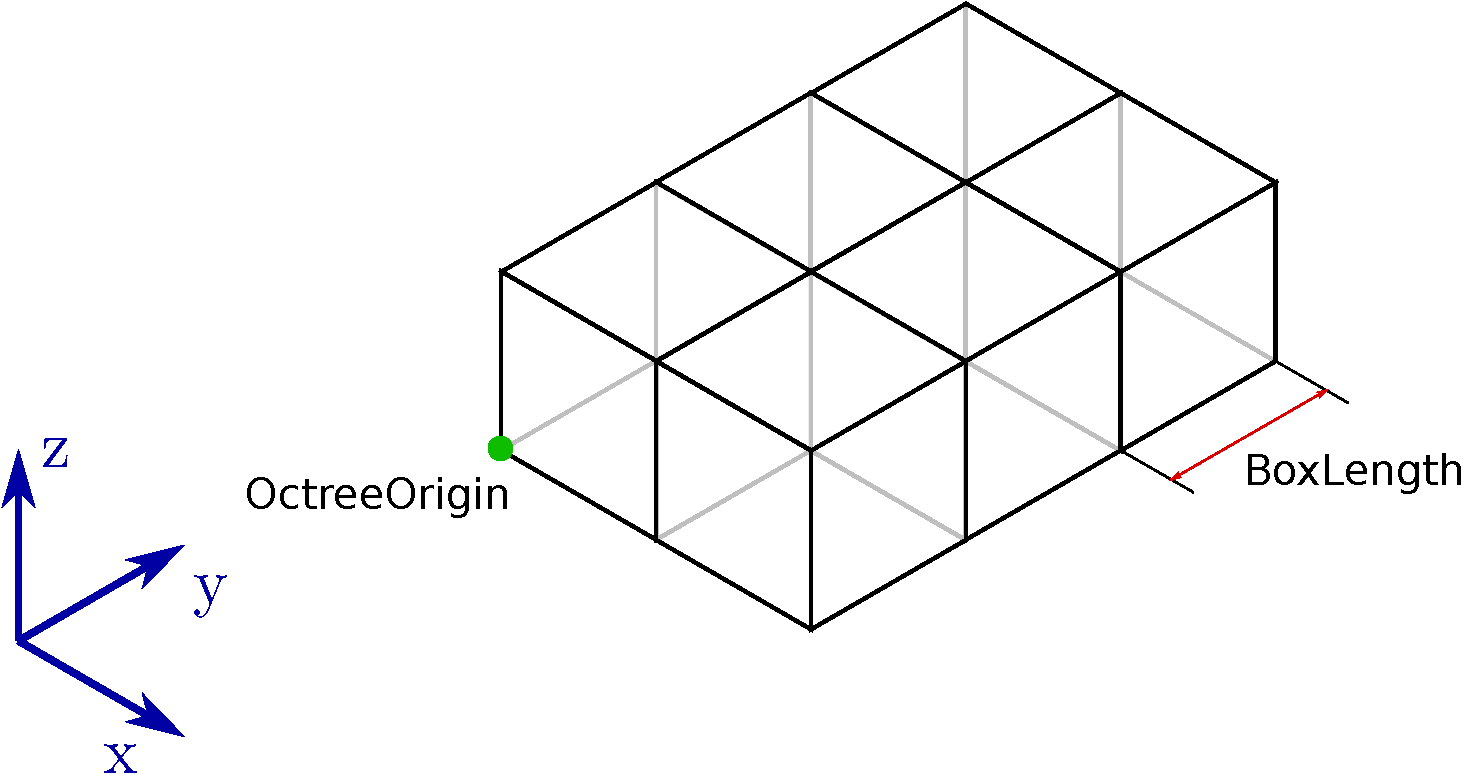
\includegraphics[width=.7\textwidth]{boxes}
\caption{System of cube boxes to compose the first level of the octree. 
In green is highlighted the origin of the octree, from which two rows of 
boxes in x, three in y and one in z starts, corresponding to \param{n_box} = (/2, 3, 1/). 
In red is highlighted the length of each cube side, \param{box_length}}
\label{fig:boxes1}
\end{figure}




\section{Time Stepping}
\label{sec:Time_Stepping}
The simulation is started from parameter \param{tstart} 
(unless restarting from a previous solution and not resetting time) 
and ends at \param{tend} after a certain number of timesteps. 
The user must provide the parameters \param{tstart}, \param{tend} 
and alternatively the number of timesteps (\param{timesteps}) between 
them or the size of the timesteps (\param{dt}). The non specified 
parameter is computed during the execution.

When specifying the number of timesteps, the interval between the 
starting time (or re-starting time) and the end time is divided in 
a number \param{timesteps} of equal intervals, and then \param{timesteps}+1 
steps are executed, counting also the starting one.

When specifying the timestep length \param{dt}, the smallest number of 
steps to get to \param{tend} is executed. If the time interval cannot be 
divided into an integer number of timesteps, all the timesteps will be 
executed anyway with a timestep length of \param{dt}, and the last timestep 
will be shorter to arrive precisely at \param{tend}. It must however be 
noted that DUST is not designed at the moment to handle variable timestep 
lengths, for this reason in few particular unsteady configurations, this 
shorter timestep could lead to small fluctuations of the loads just in the 
last timestep. To avoid this issue use a \param{dt} which lead to a precise 
number of timesteps or prescribe the number of timesteps instead of the 
timestep length (or discard the results of the last step). 

\section{Models Parameters Choice}
\label{sec:Solver_ParametersChoice}
In the previous section \ref{sec:Solver_InputFile} all the available 
parameters for the \DUST{} solver have been listed. While the brief 
description in most of the cases is enough to describe the simple 
functioning of the parameters, for some model parameters is necessary 
a more comprehensive discussion. 

\paragraph{Vortex Models Parameters}
%\textcolor{red}{Rewrite! or cancel it}

In \DUST{} all the description of both the surface elements and 
the wake relies (also) on vortex models. The vortex particles 
represent a small vortex unit, lifting lines are represented by 
a single vortex, panel wakes, vortex lattices and surface panels 
all have a uniform distribution of doublets, which is equivalent 
to a vortex ring along the sides of such panels. 

The velocity induced by vortexes decreases with a certain power 
of the distance from the vortex ($1/r$ in two dimensions, $1/r^2$ in three), 
which means that while at higher distances the induced velocity becomes 
small, for distances approaching zero the velocity becomes very high 
and eventually singular. This model is completely irrotational, with 
all the vorticity confined in a point/line, but is clearly not physical, 
and for this reason it is necessary to regularize the induced velocity 
in the proximity of the vortex. If in the case of the panels this can 
be seen merely as a regularization, in the case of the vortex particles 
the use of a regularized core is necessary to have a rotational volume 
for each particle which is able to represent the vorticity field generated 
by the wake. 

Starting precisely from this consideration, it is advisable to set the 
parameter \param{vortex_rad}, which is the radius of the Rosenhead 
regularized core employed for the vortex particles, to a value which
allow the generated particles to represent the whole generated vorticity 
field, by slightly overlapping one another. This can be done for example 
by setting \param{VotexRad} equal to the (average) length of the trailing 
edge element sides, where the particles are first generated and spaced.

Since the generation of the particles from the trailing edges sets somehow 
the spacing, and the resolution, of the vortical phenomena, the radius of 
the vortex model of the panels, \param{rankine_rad} should be chosen at least 
in the same order of magnitude of \param{vortex_rad}. The vortex 
regularization performed on the panels is the classical Rankine one. 
Since it is expected that the vortical phenomena on surfaces are more 
confined than in the wake the user might want to take a little smaller 
radius for the surface panels than the particles one, however remaining 
in the same order of magnitude. Too small radii might lead to not physical, 
too strong interactions with close particles or panels.

Eventually for the panels the parameter \param{cutoff_rad} sets a radius 
underneath which the interaction is set to zero, to avoid any kind of 
modelling when a point is essentially coinciding with the vortex. 
This parameter should be set \emph{much smaller} than \param{rankine_rad}. 


\section{Reference frames}
\label{sec:Solver_ReferenceFrames}

The reference frames are the basis for both the placement of the geometry 
components in the space and for the definition of their movement.  
Reference frames are handled by the solver, which reads them from 
a separate input file, indicated in the solver input file, file 
\ref{file:dust.in}. Before detailing the inputs for the reference 
frames file it is important to understand how reference frames work 
inside DUST. %(more details are presented in the Theory Manual).

Reference frames are defined hierarchically from a base reference frame. 
The base reference frame is called "0" and cannot be defined, 
is a standard right-nanded Cartesian reference frame and is defined 
inside DUST. Starting from the base reference frame all the necessary 
reference frames can be defined. 

It is important to stress that the base reference frame it is not 
defined upon any other implied reference frame and thus has no implied 
orientation with respect to anything else. Instead it is just the definition 
of the three axis x-y-z upon which all the other reference frames, geometrical 
components, parameters are defined. The user can give any meaning to the three 
axis, e.g. x horizontal towards rear, y horizontal towards right and z vertical 
upward, but also x front, y up and z right. The user must be then consistent 
with the inputs, both in terms of geometry and for example free stream velocity, 
but there is no implied orientation in the base reference.

All the following reference frames are defined upon another reference frame, 
called "parent" reference frames. Obviously the parent reference frame must 
always be defined, so that all the branches of the tree defined by the multiple 
reference frame can be traversed back to the base reference frame. The relative 
positioning of two reference frames with respect to the base one is depicted in 
figure \ref{fig:references1}. The use of multiple reference frames allows to 
position a geometrical entity, with its own local coordinates, in any position 
of the domain, and in any relative position with respect to the other components, 
in a logical way.  An example of references file, for static references is 
presented in file \ref{file:references_static.in}. 

\begin{figure}
\centering
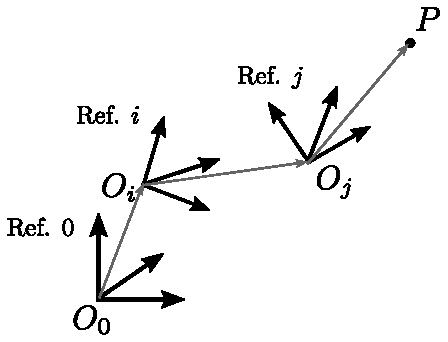
\includegraphics[width=.7\textwidth]{references1}
\caption{Positioning of relative reference frame}
\label{fig:references1}
\end{figure}

\begin{inputfile}[frame=single, caption={references\_static.in}, 
    label={file:references_static.in}]
!!!!!!!!!!!!!!!!!!!!!!!!!!!!!!!!!!!!!!!!!!!!!!!!!!!!!!!!!!!!!!!!!!!!!!!!!!!!!!!
reference_tag = root
parent_tag = 0
origin = (/0.0, 0.0, 0.0/)
orientation = (/1.0,0.0,0.0, 0.0,1.0,0.0, 0.0,0.0,1.0/)
multiple = F
moving = F

!!!!!!!!!!!!!!!!!!!!!!!!!!!!!!!!!!!!!!!!!!!!!!!!!!!!!!!!!!!!!!!!!!!!!!!!!!!!!!!
reference_tag = first
parent_tag = Root
origin = (/10.0, 2.0, 4.0/)
orientation = (/0.0,1.0,0.0, 0.0,0.0,1.0, 1.0,0.0,0.0/)
multiple = F
moving = F

!!!!!!!!!!!!!!!!!!!!!!!!!!!!!!!!!!!!!!!!!!!!!!!!!!!!!!!!!!!!!!!!!!!!!!!!!!!!!!!
reference_tag = second
parent_tag = Root
origin = (/0.0, 0.0, 0.0/)
orientation = (/0.999941,0.0,-0.010859, 0.0,1.0,0.0, +0.010859,0.0,0.999941/)
multiple = F
moving = F
\end{inputfile}
The details of the parameters are:
\begin{itemize}
\item \param{reference\_tag}: \textit{required:} yes. \textit{multiple:} yes. 
\textit{type:} string.

The tag is a unique identifier of the reference frame, it is a string and is 
referenced by the geometry component and other reference frames. All tags are 
valid except for "0" which is reserved by the base reference frame. 

The number of references tags declares the number of reference frames defined.

\item \param{parent\_tag}: \textit{required:} yes, in same number as \param{reference\_tag}. 
\textit{multiple:} yes. \textit{type:} string.

Declares the reference frame upon which the current reference frame is defined. 
The valid values are all the other reference frames defined in the input file 
(also later in the file) and "0". 

\item \param{origin}: \textit{required:} yes, in same number as \param{reference\_tag}. 
\textit{multiple:} yes. \textit{type:} real array of length 3.

origin of the current reference frame, in coordinates of the parent reference frame 
(not the global ones). 

\item \param{orientation}: \textit{required:} yes, in same number as \param{reference\_tag}. 
\textit{multiple:} yes. \textit{position:} must follow \param{origin} 
\textit{type:} real array of length 9.

orientation of the current reference frame with respect to the previous one. 
Considering a Fortran filling order (fastest cycling index is the row one), 
the 9 component vector forms a matrix with the vectors of the current base 
in the components of the parent base, by columns. In other words the first 
three coefficients represent the components of the x axis of the current frame 
in the parent frame, and so on for y and z axis. 

\item \param{multiple}: \textit{required:} yes, in same number as \param{reference\_tag}. 
\textit{multiple:} yes. \textit{type:} logical.
Is the reference frame multiple? 

\item \param{moving}: \textit{required:} yes, in same number as \param{reference\_tag}. 
\textit{multiple:} yes. \textit{type:} logical.
Is the reference frame moving with respect to the parent? 
\end{itemize}

\section{Moving reference frames}
Special input is required when a reference frame is moving or is multiple, 
in which case a special grouping keyword is required. 
As shown in file \ref{file:references_moving.in} if the parameter \param{moving} 
is set to true, it must be followed by the grouping parameter \param{motion} 
in which the definition of the motion is provided. 

All the motions in DUST are provided as a translation of a pole and a 
rotation around an axis passing from the pole, as depicted in figure 
\ref{fig:references2}. The motion of the pole can be defined in terms 
of position or velocity. Both can be described with some simple functions 
or from a time history from a data file.
In the same way the rotation around an axis can be defined in terms 
of angle or rotation rate, and with simple functions or data input.

The simple functions are either a constant value, or a sinusoidal function 
of time defined as
\begin{equation}
f(t) = A \sin{\omega t + \phi} + r 
\end{equation}
where $A$ is the amplitude, $\omega$ the pulsation, $\phi$ the phase and $r$ an offset. 

\begin{inputfile}[frame=single, caption={references\_moving.in}, 
    label={file:references_moving.in}]
!!!!!!!!!!!!!!!!!!!!!!!!!!!!!!!!!!!!!!!!!!!!!!!!!!!!!!!!!!!!!!!!!!!!!!!!!!!!!!!
reference_tag = moving
parent_tag = 0
origin = (/0.0, 1.0, 0.0/)
orientation = (/1.0,0.0,0.0, 0.0,1.0,0.0, 0.0,0.0,1.0/)
multiple = F
moving = T
motion = {
  pole = {
    input      = position                           
    input_type = simple_function
    function   = (/  0  ,  0  ,  0  /)
    !file       = xxx.dat
    amplitude  = 0.00
    vector     = (/ 0.0 , 0.0 , 0.0 /)
    omega      = (/ 0.0 , 0.0 , 0.0 /)
    phase      = (/ 0.0 , 0.0 , 0.0 /)
    offset     = (/ 0.0 , 0.0 , 0.0 /)
    !position_0 = ...
  }
  rotation   = {
    input      = position
    input_type = simple_function
    !file = ...
    function   =  1      
    Axis       = (/ 0.0 , 1.0 , 0.0 /)  
    amplitude  = 0.1    
    omega      = 1.2566  
    phase      = 0.0  
    offset     = 0.0  
    psi_0      = 0.0           
  }
}
\end{inputfile}

The details of the parameters inside the \param{motion} group are:
\begin{itemize}
\item \param{pole}: \textit{required:} yes. \textit{multiple:} 
not inside each \param{motion} group.

Grouping keyword containing the specification of the pole motion, 
the pole motion parameters are

	\begin{itemize}
	\item \param{input}: \textit{required:} yes. \textit{multiple:} 
    not inside each \param{pole} group. \textit{type:} string.
    
    In which way motion is imposed, can be \opt{position} or \opt{velocity}
    
    \item \param{input\_type}: \textit{required:} yes. \textit{multiple:} 
    not inside each \param{pole} group. \textit{type:} string.
    
    type of input, can be \opt{simple\_function} or \opt{from\_file}
    
    \item \param{function}: \textit{required:} yes if \param{input\_type} 
    is \opt{simple\_function}. \textit{multiple:} not inside each \param{pole} 
    group. \textit{type:} integer array of length 3.
    
    type of function to be imposed, at the moment \opt{0} is for a constant 
    function and \opt{1} is for a sinusoidal function. An array of three 
    components is expected, one for each direction of the pole motion.    

        \item \param{file}: \textit{required:} yes if \param{input\_type} 
        is \opt{from\_file}. \textit{multiple:} not inside each \param{pole} 
        group. \textit{type:} string.
        
        name of the file where the time history is of the motion 
        (position or velocity) is stored. The file is supposed to have 
        4 columns, the first containing a series of time values adequate 
        for the simulation time, and the following three the three components 
        of the pole motion. 
        
    \item \param{amplitude}: \textit{required:} no, used only if \param{input\_type}     
    is \opt{simple\_function}. \textit{multiple:} not inside each \param{pole} group. 
    \textit{default:} 1.0 \textit{type:} real.
    
    Collective amplitude of the motion, applied to all the three components of the motion    
    
     \item \param{vector}: \textit{required:} no, used only if \param{input\_type} 
     is \opt{simple\_function}. \textit{multiple:} not inside each \param{pole} group. 
     \textit{default:} (/1.0, 1.0, 1.0/) \textit{type:} real array of length 3.
    
    Relative amplitude of the motion for each component
    
    \item \param{omega}: \textit{required:} no, used only if \param{input\_type} 
    is \opt{simple\_function}. \textit{multiple:} not inside each \param{pole} group. 
    \textit{default:} (/1.0, 1.0, 1.0/) \textit{type:} real array of length 3
    
    Pulsation of each sinusoidal motion. Considered only if input is 
    \opt{simple\_function} and only for the components with sinusoidal functions.
    
    \item \param{phase}: \textit{required:} no, used only if \param{input\_type} 
    is \opt{simple\_function}. \textit{multiple:} not inside each \param{pole} group. 
    \textit{default:} (/0.0, 0.0, 0.0/) \textit{type:} real array of length 3.
    
    phase of each sinusoidal motion. Considered only if input is \opt{simple\_function} 
    and only for the components with sinusoidal functions.
    
    \item \param{offset}: \textit{required:} no, used only if \param{input\_type} 
    is \opt{simple\_function}. \textit{multiple:} not inside each \param{pole} group. 
    \textit{default:} (/0.0, 0.0, 0.0/) \textit{type:} real array of length 3.
    
    Constant offset (position/velocity) for each component of the pole motion
    
    \item \param{Position\_0}: \textit{required:} no, used only if \param{input\_type} 
    is \opt{simple\_function}. \textit{multiple:} not inside each \param{pole} group. 
    \textit{default:} (/0.0, 0.0, 0.0/) \textit{type:} real array of length 3
    
    Starting position of the pole in the three component, considered only if 
    \param{input} is \opt{velocity}
    
	\end{itemize}

\item \param{rotation}: \textit{required:} yes. \textit{multiple:} not inside each 
\param{motion} group.

Grouping keyword containing the specification of the rotation, which parameters are:

	\begin{itemize}
	\item \param{input}: \textit{required:} yes. \textit{multiple:} not inside each 
    \param{rotation} group. \textit{type:} string.
    
    In which way the rotation is imposed, can be \opt{position} for imposing an angle  
    or \opt{velocity} for imposing a rotation rate
    
    \item \param{input\_type}: \textit{required:} yes. \textit{multiple:} not inside 
    each \param{rotation} group. \textit{type:} string.
    
    type of input, can be \opt{simple\_function} or \opt{from\_file}
    
    \item \param{function}: \textit{required:} yes if \param{input\_type} is 
    \opt{simple\_function}. \textit{multiple:} not inside each \param{rotation} group. 
    \textit{type:} integer.
    
    type of function to be imposed, at the moment \opt{0} is for a constant function 
    and \opt{1} is for a sinusoidal function.
    
        \item \param{file}: \textit{required:} yes if \param{input\_type} is 
        \opt{from\_file}. \textit{multiple:} not inside each \param{rotation} group. 
        \textit{type:} string.
        
        name of the file where the time history is of the rotation 
        (angle or rotation rate) is stored. The file is supposed to have 2 columns, 
        the first containing a series of time values adequate for the simulation time, 
        and the following the rotation around the axis. 
        
    \item \param{Axis}: \textit{required:} yes. \textit{multiple:} not inside each 
    \param{rotation} group. \textit{type:} real array of length 3.
    
    orientation of the rotation axis, in the parent reference frame. The rotation 
    axis keeps a constant orientation in the parent reference frame and always passes 
    through the pole during its motion
    
    \item \param{amplitude}: \textit{required:} no, used only if \param{input\_type} 
    is \opt{simple\_function}. \textit{multiple:} not inside each \param{rotation} group. 
    \textit{default:} 1.0 \textit{type:} real.
    
    Collective amplitude of the rotation 
    
    \item \param{omega}: \textit{required:} no, used only if \param{input\_type} 
    is \opt{simple\_function}. \textit{multiple:} not inside each \param{rotation} group. 
    \textit{default:} 1.0 \textit{type:} real.
    
    Pulsation of the sinusoidal motion. Considered only if \param{input} is 
    \opt{simple\_function} and \param{input\_type} is a sinusoidal function.
    
        \item \param{phase}: \textit{required:} no, used only if 
        \param{input\_type} is \opt{simple\_function}. \textit{multiple:} not 
        inside each \param{rotation} group. \textit{default:} 0.0 \textit{type:} real.
    
    phase of the sinusoidal motion. Considered only if \param{input} is 
    \opt{simple\_function} and \param{input\_type} is a sinusoidal function.
    
    \item \param{offset}: \textit{required:} no, used only if \param{input\_type} 
    is \opt{simple\_function}. \textit{multiple:} not inside each \param{rotation} group. 
    \textit{default:} 0.0 \textit{type:} real.
    
    Constant offset of rotation or rotation rate
    
    \item \param{Psi\_0}: \textit{required:} no, used only if \param{input\_type} 
    is \opt{simple\_function}. \textit{multiple:} not inside each \param{rotation} group. 
    \textit{default:} 0.0 \textit{type:} real.
    
    Starting angle of the rotation, considered only if \param{input} is \opt{velocity}
    
	\end{itemize}

\end{itemize}

\begin{figure}
\centering
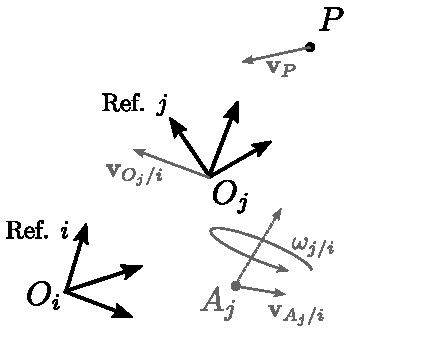
\includegraphics[width=.7\textwidth]{references2}
\caption{Velocity of relative reference frame}
\label{fig:references2}
\end{figure}

\section{Multiple reference frames}
To ease the setup of rotors in terms of reference frames and motions, 
a special set of instructions have been developed for the reference frames. 
Declaring a reference frame multiple, a single component is replicated n times 
in a special set of multiple, automatically generated reference frames. 
While there is possibility to expansion towards different types of multiple 
reference frames, at the moment multiplicity is employed only for rotors: an 
example input file with a reference frame for a rotor is given in file 
\ref{file:references_rotor.in}. 

\begin{inputfile}[frame=single, caption={references\_rotor.in}, label={file:references_rotor.in}]
!!!!!!!!!!!!!!!!!!!!!!!!!!!!!!!!!!!!!!!!!!!!!!!!!!!!!!!!!!!!!!!!!!!!!!!!!!!!!!!
reference_tag = Rotor01
parent_tag = Root
origin = (/0.0, 0.0, 0.0/)
orientation = (/1.0,0.0,0.0, 0.0,1.0,0.0, 0.0,0.0,1.0/)
moving = F
multiple = T
multiplicity = {
  mult_type = rotor
  n_blades = 4
  rot_axis = (/0.0, 0.0, 1.0/)
  rot_rate = 6.28318530717959 !2*pi, T=1
  psi_0 = 0.0
  hub_offset = 0.0

  n_dofs = 3
  dof = {
    hinge_type = Flap
    hinge_offset = (/ 0.0 , 0.032432 , 0.0 /)
    Collective  =  3.0     ! deg
    cyclic_ampl =  0.0     ! deg
    cyclic_phas =  0.0     ! deg
  }
  dof = {
    hinge_type = Lag
    hinge_offset = (/ 0.0 , 0.021622 , 0.0 /)
    Collective  = -10.0
    cyclic_ampl =  0.0
    cyclic_phas =  0.0
  }
  dof = {
    hinge_type = Pitch
    hinge_offset = (/ 0.0 , 0.086486 , 0.0 /)
    Collective  = 12.0
    cyclic_ampl =  0.0
    cyclic_phas =  0.0
  }

}


\end{inputfile}
Note that the rotor reference frame in file \ref{file:references_rotor.in} 
is set as not moving. This means that the starting reference frame is stationary 
(with respect to its parent) however all the other reference frames that are 
automatically generated move in order to represent the different movements of a rotor.

If in the reference frame specification the parameter \param{multiple} 
is set to true, it must be followed by a grouping keyword, \param{multiplicity}, 
which must contain the details of the multiplicity. The detailed parameters 
required in the multiplicity are:
\begin{itemize}
	\item \param{mult_type}: \textit{required:} yes. \textit{multiple:} 
    not inside each \param{multiplicity} group. \textit{type:} string.
    
	type of multiplicity. At the moment only \opt{rotor} is enabled.
    
    \item \param{N\_Blades}: \textit{required:} yes if \param{mult_type} 
    is \opt{rotor}. \textit{multiple:} not inside each \param{multiplicity} group. 
    \textit{type:} integer.
    
    Number of blades of the rotor. It is also the number of time the geometrical 
    component associated with the reference frame will be multiplied in the domain. 
    
    \item \param{Rot\_Axis}: \textit{required:} yes if \param{mult_type} is \opt{rotor}. 
    \textit{multiple:} not inside each \param{multiplicity} group. 
    \textit{type:} real array of length 3.
    
    Axis of rotation of the rotor, with respect to the current reference frame
    
    \item \param{Rot\_Rate}: \textit{required:} yes if \param{mult_type} is \opt{rotor}. 
    \textit{multiple:} not inside each \param{multiplicity} group. \textit{type:} real.
    
    rotation rate of the blades around the rotation axis. 
    The rotation of the rotor is kept constant.
    
    \item \param{Psi\_0}: \textit{required:} yes if \param{mult_type} is \opt{rotor}. 
    \textit{multiple:} not inside each \param{multiplicity} group. \textit{type:} real.
    
    Starting angle of the rotor at the beginning of the simulation
    
    \item \param{Hub\_Offset}: \textit{required:} yes if \param{mult_type} is \opt{rotor}. 
    \textit{multiple:} not inside each \param{multiplicity} group. \textit{type:} real. 
    
    offset from the rotation pole (the origin of the multiple reference frame) of the beginning of the chain of reference frames for each blade. It is constant and does not imply any secondary motion, can be used to represent the central part of the rotor axis assembly. 
    
    \item \param{N\_dofs}: \textit{required:} yes if \param{mult_type} is \opt{rotor}. 
    \textit{multiple:} not inside each \param{multiplicity} group. \textit{type:} integer.
    
    Number of additional degrees of freedom of each blade, generally representing 
    a movement around one of the blades hinges
    
    \item \param{dof}: \textit{required:} yes if \param{N\_dofs} is greater than zero. 
    \textit{multiple:} yes, in the number defined by \param{N\_dofs}. 
    
    Grouping keyword containing the details about geometry and movement of 
    one additional degree of freedom. The degrees of freedom are connected in 
    a chain according to the order in which are defined. A representation of 
    the chain of degrees of freedom is presented in figure \ref{fig:multiple_refs}.
    
    \begin{itemize}
    \item \param{hinge\_Type}: \textit{required:} yes. \textit{multiple:} 
    not inside each \param{dof} group. \textit{type:} string.
    
    type of hinge considered, affecting the axis of rotation of the hinge 
    movement with respect to the rotor axis, can be \opt{Flap},\opt{Lag}, or \opt{Pitch}.
    
    \item \param{hinge\_Offset}: \textit{required:} yes. \textit{multiple:} 
    not inside each \param{dof} group. \textit{type:} real array of length 3.
    
    offset of the hinge rotation axis with respect to the previous hinge or 
    the rotor hub (axis + hub offset).
    
    \item \param{Collective}: \textit{required:} yes. \textit{multiple:} not 
    inside each \param{dof} group. \textit{type:} real.
    
    Collective (constant during rotation) angle of rotation (in degrees) of 
    the degree of freedom.
    
    \item \param{Cyclic\_Ampl}: \textit{required:} yes. \textit{multiple:} 
    not inside each \param{dof} group. \textit{type:} real.
    
    Cyclic (sinusoidal during rotation) angle of rotation (in degrees) of 
    the degree of freedom.
    
    \item \param{Cyclic\_Phas}: \textit{required:} yes. \textit{multiple:} 
    not inside each \param{dof} group. \textit{type:} real.
    
    phase of the cyclic movement, in degrees, with respect to the rotor rotation. 
    
    \end{itemize}
\end{itemize}

\begin{figure}
\centering
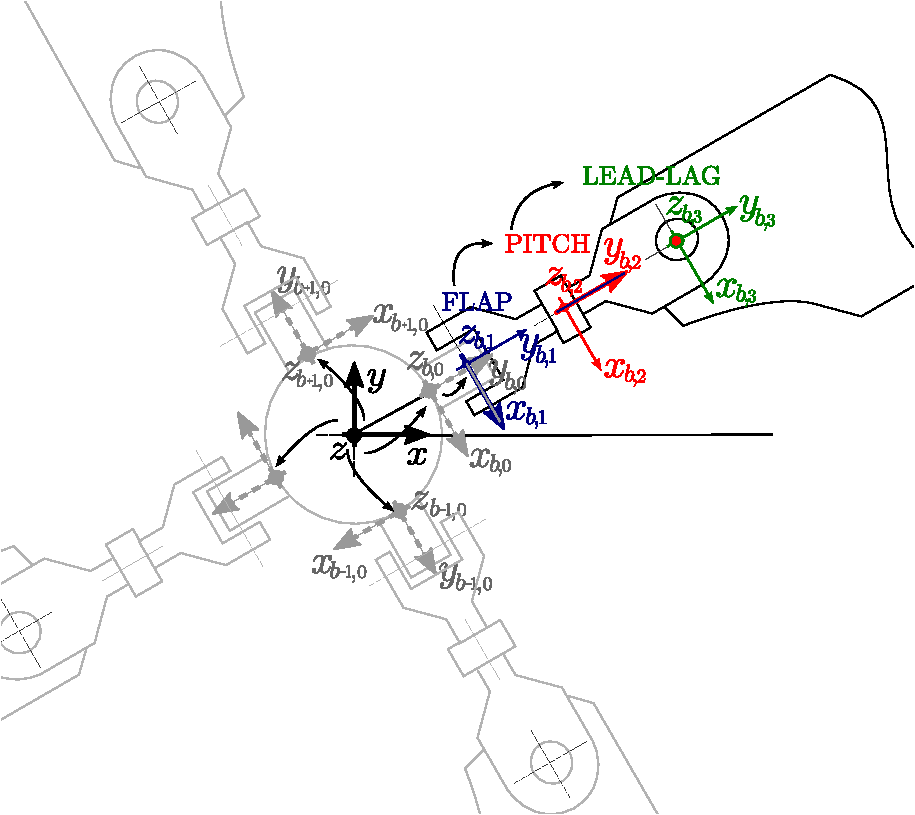
\includegraphics[width=.7\textwidth]{rotor_scheme}
\caption{multiple reference frames in a rotor}
\label{fig:multiple_refs}
\end{figure}

\section{Dimensional Units}
\label{sec:Dimensional_Units}

In the present section the dimensional units, normalization (or the lack of it) 
in \DUST{} will be discussed.

All the equations, models, inputs, outputs etc. in the code are \textbf{dimensional}. 
This does not mean that they are required to be in a specific dimensional unit, 
but only that \textbf{no sort of non-dimensionalization is performed in the code}. 
The user is fully resposible for the scaling (or not) of his inputs, and as a 
consequence of the outputs. 

More in detail the core of \DUST{} solves the potential equations, which are a 
simplified version of the incompressible Euler equations. Such equations do not 
depend on a scaling parameter (such as Mach or Reynolds for compressible Navier-Stokes) 
so their (scaled) results are independent on the scaling employed. Three possible 
approaches at the scaling of the variables and results are given in examples 
\ref{ex:pot-dim},\ref{ex:pot-nondim} and \ref{ex:pot-part}. 

\begin{example}[Potential case, fully dimensional]
\label{ex:pot-dim}
Consider a isolated wing with span $b = 20 m$ and chord $c = 2 m$ flying at 
$U = 60 m/s$ in air with density $\rho = 1.225 kg/m^3$. 

The user can take a completely dimensional approach and insert (or build) 
the geometry in the correct size in meters, and impose a free stream velocity 
and density corresponding to the real flight conditions. In this case the results, 
for example in terms of loads, will be in the same units set employed in the inputs, 
$L [N]$. To obtain the loads coefficient then the user must non-dimensionalize the 
results employing the appropriate reference quantities used in the computations:
\begin{equation*}
    C_L = \frac{L}{1/2 \rho U^2 b c} = \frac{L}{1/2 \cdot 1.225  \cdot 60^2 \cdot 20 \cdot 2}
\end{equation*}
\end{example}

\begin{example}[Potential case, fully scaled]
\label{ex:pot-nondim}
Starting from the conditions of example \ref{ex:pot-dim}, a user might want 
to re-scale all the quantities with respect to scaling units. For example, 
the geometry might be scaled by the span, giving $b' = b/b = 1$, $c'=c/b=0.1$ 
and introduced scaled from the mesh generator, scaled in the pre-processor or 
built parametrically already scaled. The velocity might be scaled on the free 
stream one, specifying directly $U'=U/U=1$, as well as the density $\rho' = \rho/\rho = 1$. 

With these parameters as input, the output would be scaled accordingly, 
leding for example to the scaled loads $L'$. These outputs, being scaled, 
are not numerically equal to the ones obtained in example \ref{ex:pot-dim}, 
however they can be on the one hand scaled back to the real ones employing 
the inverse scaling used for the inputs, or on the other hand if only the 
non-dimensional coefficients are sought they can be obtained using the scaled 
reference quantities:
\begin{equation*}
    C_L = \frac{L'}{1/2 \rho' U'^2 b' c'} = \frac{L'}{1/2 \cdot 1  \cdot 1^2 \cdot 1 \cdot 0.1}
\end{equation*}
When non-dimensionalized on the appropriate reference quantities the 
non-dimensional coefficients have always the same values.
\end{example}

\begin{example}[Potential case, partially scaled]
\label{ex:pot-part}
While in example \ref{ex:pot-nondim} all the quantities have been scaled 
with respect to some scaling quantity, the user can choose to use different 
quantities, or to scale only some of the quantities. For example, 
the user might want to keep the geometry from the CAD in meters, 
$b = 20 m$, $c = 2 m$ and scale the flight conditions for ease of use, 
$U'=U/U=1$, $\rho' = \rho/\rho = 1$. 

The results $L''$ are going to be again scaled, in a different way than 
in example \ref{ex:pot-nondim}, and the non-dimensional coefficient can 
be retrieved using the reference quantities employed in the computation:
\begin{equation*}
    C_L = \frac{L''}{1/2 \rho' U'^2 b c} = \frac{L''}{1/2 \cdot 1  \cdot 1^2 \cdot 20 \cdot 2}
\end{equation*}
\end{example}

It must however be stressed that when talking about scaling of the inputs 
and non-dimensionalization of the results, these operations are left to the 
user to be carried out independently before and after the execution of \DUST{}. 
To maintain complete usage flexibility, it is not possible to introduce any 
explicit scaling or non-dimensionalizing unit. 
When using certain features of the code (lifting lines, 
vorticity diffusion, separations etc.) the effects of viscosity 
and compressibility are simulated in different manners. 
To account for the right flow conditions it is necessary 
to specify the parameters governing the viscous and 
compressibility phenomena, i.e. the dynamic viscosity 
$\mu$ and the speed of sound $c$ in the input file. 
In continuity with the rest of the code, the dimensional physical 
properties of the flow must be provided, rather than the non dimensional 
numbers Reynolds and Mach. It is responsibility of the user to insert 
them correctly and eventually scale them to obtain similarity of Reynolds 
and Mach with respect to the target conditions. Examples on how to achieve 
that in different conditions are presented in example \ref{ex:rema-scaling}.

\begin{example}[Ways to determine physical properties]
\label{ex:rema-scaling}
Depending on the cases, the physical properties of the fluid to be given as input might be:
\begin{itemize}
    \item Already known and inserted as they are, if all the other reference 
    quantities have not be scaled
    \item Obtained from the original ones, keeping Reynolds and Mach number 
    equal, if some of the reference quantities were scaled:
    \begin{equation*}
        \frac{\rho U L}{\mu} = \frac{\rho' U' L'}{\mu'} \quad \rightarrow \quad \mu' = \mu \frac{\rho' U' L'}{\rho U L}
    \end{equation*}
    \begin{equation*}
        \frac{U}{c} = \frac{U'}{c'} \quad \rightarrow \quad c' = c \frac{U'}{U}
    \end{equation*}
    \item Obtained from the non-dimensional parameters, if those are known rather 
    than the properties of the fluid:
    \begin{equation*}
        Re = \frac{\rho' U' L'}{\mu'} \quad \rightarrow \quad \mu' = \frac{\rho' U' L'}{Re}
    \end{equation*}
    \begin{equation*}
        Ma = \frac{U'}{c'} \quad \rightarrow \quad c' = \frac{U'}{M}
    \end{equation*}
\end{itemize}
\end{example}

Finally, the reference pressure given as input is used as reference, 
free stream pressure, and does not affect the results except for a 
constant offset in the pressure field output. Loads are computed 
integrating on a closed surface and so are not affected by a constant 
offset on pressure. Knowing the reference pressure used as input, 
it is possible to retrieve the local coefficient of pressure:
\begin{equation*}
    C_p(\vec{x}) = \frac{P(\vec{x})-P_{ref}}{1/2 \rho U^2}
\end{equation*}
where $P(\vec{x})$ is the local pressure from the results, $P(\vec{x})$ 
is the reference pressure given as input and $\rho, U$ are the reference 
quantities employed during the simulation. 


\section{Debug Levels}
\label{sec:Solver_DebugLevels}

As discussed in section \ref{sec:Solver_InputFile} in the solver input 
file it is possible to set the parameter \param{debug\_level} which selects 
the verbosity of the output of the code. The level is selected choosing an 
integer number, and it is cumulative: selecting a certain value the user gets 
the additional output given at that value \emph{and} all the outputs at the lower levels. 
As a rule of thumb the debug levels up to 10 generate increasing levels of 
verbosity in the screen outputs, while increasing levels over 10 generate 
additional outputs saved in files, in the appropriate \param{basename\_debug} path. 
The current effects of the debug level are presented in table \ref{tab:debug_level}. 
Be aware that the debug file output is mainly targeted for development work, and its 
content is susceptible to sudden and undocumented changes. 

\begin{table}[]
\centering
\begin{tabular}{@{}rl@{}}
\toprule
Debug Level & Effects \\ \midrule
<0            & Almost no screen output, useful just for batch runs        \\
1             & Minimal screen output        \\
3             & Standard screen output information         \\ 
5             & Verbose screen output (fmm data etc.)\\
7             & Extra warnings and diagnostics, can lead to false negative warnings\\ 
8             & Extra verbose output (lifting lines data etc.)\\\midrule
15            & Output minimal geometry in ascii files \\
15            & Output extended geometry in ascii files \\
20            & Output the solution in ascii files \\
50            & Output the full linear system in ascii files\\
\bottomrule
\end{tabular}
\caption{\param{debug\_level} levels and their effects}
\label{tab:debug_level}
\end{table}

\section{Output Files}
\label{sec:Solver_Output_Files}

When running the solver, a certain number of hdf5 binary files are generated, 
in the location specified by \param{basename}. Two main type of files are generated:
\begin{itemize}
    \item \opt{basename}\_geo.h5: a file containing the geometry of the simulation, 
    which is similar to the input given to the solver, with some additions related 
    to the single simulation.
    \item \opt{basename}\_res\_XXXX.h5: a number of result files obtained during 
    the simulation, printed at the frequency specified in the input file. 
\end{itemize}
